

\documentclass[12pt,a4paper]{article}
\newcommand\persiangloss[2]{#1\dotfill\lr{#2}\\}
\usepackage{graphicx}
\usepackage{xcolor}
\usepackage{listings}
\usepackage{indentfirst}
\usepackage{float}
\usepackage[pagebackref=false,colorlinks,linkcolor=blue,citecolor=magenta]{hyperref}
\usepackage{xepersian}
\settextfont{XB Niloofar}
\definecolor{vgreen}{RGB}{104,180,104}
\definecolor{vblue}{RGB}{49,49,255}
\definecolor{vorange}{RGB}{255,143,102}

\lstdefinestyle{verilog-style}
{
	language=C,
	basicstyle=\small\ttfamily,
	keywordstyle=\color{vblue},
	identifierstyle=\color{black},
	commentstyle=\color{vgreen},
	numbers=left,
	numberstyle=\tiny\color{black},
	numbersep=10pt,
	tabsize=8,
	moredelim=*[s][\colorIndex]{[}{]},
	literate=*{:}{:}1
} 



\begin{document}
	\thispagestyle{empty}
	\vspace*{0mm}
	\centerline{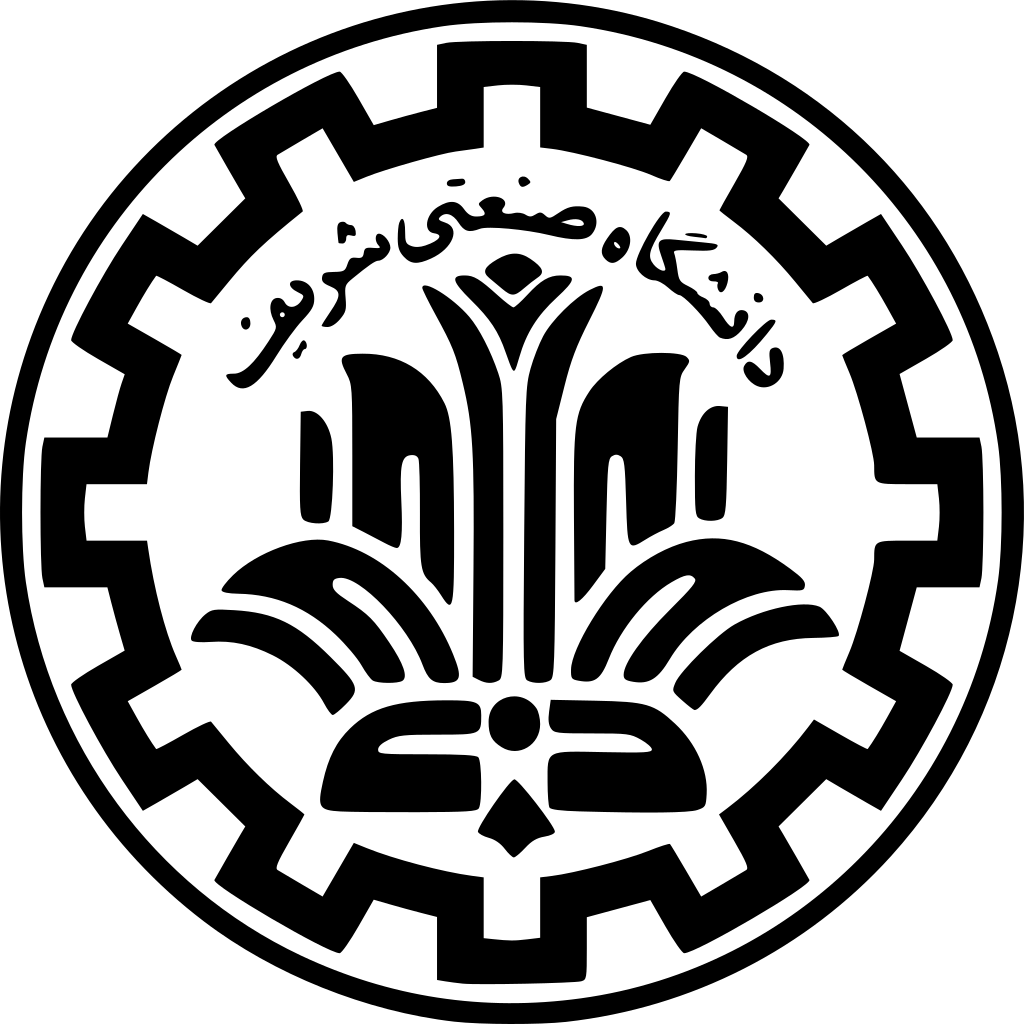
\includegraphics[height=4cm]{logo.png}}
	\vspace*{5mm}
	\begin{center}
		{\Huge
			لوستر هوشمند
		}
		\\[1cm]
		آزمایشگاه سخت‌افزار
		\\[1cm]
		دانشکده مهندسی کامپیوتر
		\\[4cm]
		{\large
			محمدرضا عبدی ۹۷۱۱۰۲۸۵
			
			حمیدرضا کامکاری ۹۷۱۱۰۱۷۷
			
			یگانه قره‌داغی 97106216
		}
		\\[5cm]
		خرداد ۱۴۰۱
	\end{center}
	\newpage
		\section*{چکیده}
	
	روند خودکار سازی فعلی خانه‌ها قدمی مهم برای کاهش مصرف بی‌اندازه برق و تسهیل زندگی افراد خانه است. انواع لوستر‌ها و تجهیزات روشنایی از جدیدترین وسایل اضافه شده به لوازم خانگی هوشمند هستند. هدف از این پروژه طراحی یک لوستر هوشمند است که بتواند به کمک یک برنامه به لوازم جانبی هوشمند دیگر (مانند تلفن‌های همراه) متصل شود و توسط آن به صورت خودکار یا دستی تنظیم شود. این دستگاه جزو یک شبکه اینترنت اشیا (\lr{Internet of Things}) است و با استفاده از یک برنامه موبایل قابل مدیریت است. 
	
	در این گزارش به توضیح قابلیت‌ها، محدودیت‌ها، قطعات و جزئیات پیاده‌سازی لوستر هوشمند در ۶ بخش می‌پردازیم.
	\newpage
	
	\tableofcontents
	
		\newpage
	
	\section{قابلیت‌های لوستر هوشمند}
	با توجه به اهداف پروژه در خودکار سازی روشنایی خانه\footnote{کاهش مصرف برق و تسهیل استفاده نسبت به لوسترهای مرسوم}، قابلیت‌های زیر برای محصول در نظر گرفته شده‌اند\footnote{جزئیات قابلیت‌ها در توصیف برنامه موبایل به صورت کامل توضیح داده‌ می‌شود.}:
	
	\begin{itemize}
		\item
		در اولین مرحله این لوستر می‌تواند به کمک سنسوری بر اساس شرایط محیطی مانند وضعیت پرده‌ها یا روشنایی طبیعی بازخورد بدهد؛ در صورت زیاد بودن شدت نور محیط، روشنایی لوستر کاهش و در صورت کم بودن شدت نور افزایش می‌یابد. میزان حساسیت نسبت به روشنایی و میزان روشنایی مورد نیاز می‌تواند بر اساس نیاز کاربر تغییر کند. به عنوان مثال پارامتر‌ اندازه اتاق می‌تواند در تنظیمات تاثیر داده شود. یعنی برای اتاق‌های بزرگتر شدت نور به هنگام روشن بودن بیشتر باشد. 
		\item
		می‌توان تنظیمات روشنایی لوستر را به صورت خودکار یا دستی تنظیم کرد. در صورت انتخاب حالت دستی، کاربر می‌تواند میزان روشنایی ثابتی را انتخاب کند.
		\item
		کاربر می‌تواند شاخه (اتاق‌های مختلف خانه) دلخواه خود را انتخاب کند و تنظیمات هر کدام از قسمت‌ها را به صورت جداگانه انجام دهد.
		\item
		کاربر می‌تواند از میان حالت‌های‌ \footnote{Mode} مختلف ارائه شده برای زیبایی یا رقص نور استفاده نماید.
		\item
		تمامی تنظیمات مذکور می‌توانند توسط یه برنامه موبایل سازگار با دستگاه‌های مبتنی بر سیستم‌عامل‌های مختلف همانند \lr{Andriod} و \lr{IOS} در لوستر اعمال شوند.
	\end{itemize}
	\newpage
	\section{محدودیت‌های اولیه لوستر هوشمند}
	
	در هنگام پیاده‌سازی و استفاده از پروژه با محدودیت‌هایی مواجه می‌شویم که در ادامه آن‌ها را تشریح می‌کنیم:
	
	\begin{itemize}
		\item
		چالش اصلی اتصال تعداد زیادی دیود ساطع نور \lr{LED\footnote{\lr{Light-emitting diode}}} با نورهای متغیر به برد برای شبیه‌سازی یک لوستر واقعی است. در نهایت با اتصال ۴۰ قطعه \lr{LED} به یک منبع خارجی ۵ ولت و کنترل آن بویسله خروجی \lr{PWM} و دو ترانزیستور (برای دو شاخه - کد این پروژه قابلیت پشتیانی از تعداد شاخه‌های بیشتر را نیز دارد) لوستر را شبیه‌سازی کردیم.
		\item
		در برخی موارد، برنامه‌های گوشی‌های هوشمند با اتصال خود به سیستم روشنایی سازگار نیستند. در این پروژه سعی شده‌است که یک برنامه موبایل سازگار با سیستم‌عامل‌های مانند \lr{Android}و \lr{IOS} مختلف برای برطرف شدن این مشکل ارائه شود.
		\item
		با وجود اینکه این موضوع کمتر و کمتر اتفاق می‌افتد، اما هر اتصال \lr{WiFi}‌ای گاهی اوقات دچار اختلال می‌شود. با توجه به اینکه لوستر هوشمند بستری بر پایه \lr{IoT} است، بدون اتصال \lr{WiFi} نمی‌توان از تنظیمات لوستر بهره برد. بنابراین پیشنهاد می‌شود که دکمه‌ها و یا کلید‌های سخت‌افزاری همچنان برای تنظیمات پایه‌ موجود باشد.
	\end{itemize}
	\newpage
	\section{قطعات مورد استفاده}
	لوستر از دو شاخه \lr{LED} تشکیل شده و میزان ولتاژ ورودی هر کدام از این شاخه‌ها از طریق پورت مربوطه روی بورد \lr{Arduino} و ترانزیستور (\lr{MOSFET IRF640}) کنترل می‌شود. برای پیاده‌سازی منطق لوستر از بورد \lr{Arduino Mega} استفاده می‌کنیم که از طریق سنسور‌های تشخیص نور (\lr{BH1750FVI}) نور محیط را تشخیص می‌دهد و بر اساس پیش‌فرض‌هاییکه در سرور \lr{IOT} چیده‌شده میزان ولتاژ خروجی‌های آنالوگ را تنظیم می‌کند. از طرفی برای اتصال به اینترنت اشیا یک سرور کوچک خانگی را روی ماژول \lr{ESP8266 ESP-01S} اجرا می‌کنیم. این سرور تنظیمات کنترل لوستر را در خود دارد و با استفاده از گوشی همراه و اتصال به آن سرور می‌توانیم این تنظیمات را کنترل کنیم. می‌توان در این پروژه از برد \lr{Arduino Uno} نیز استفاده کرد.
	
	در جدول زیر می‌توان هزینه برآورد شده قطعات و هزینه‌های پروژه را مشاهده کرد (هزینه کل معادل با 7,580,000 ریال است).
	
	\begin{table}[H]
		\centering
		\begin{tabular}{|c|c|c|}
			\hline
			هزینه     & تعداد & نام قطعه                                    \\ \hline
			700,000   & ۱     & ماژول سنجش شدت نور GY-30 با سنسور BH1750FVI \\ \hline
			۴۵۰,۰۰۰   & ۱     & ماژول ESP8266وای فای                        \\ \hline
			4,500,000 & 1     & آردوینو مگا 2560 R3                         \\ \hline
			200,000   & 1     & کابل USB به USB Type-B مخصوص آردوینو        \\ \hline
			240,000   & ۴۰    & اورل LED در دو رنگ اصلی                     \\ \hline
			70,000    & ۱     & کابل 30 سانتی نر به ماده (1  بسته 40 عددی)  \\ \hline
			700,000   & ۲     & کابل جامپر مخصوص برد بورد (بسته ۶۰ عددی)    \\ \hline
			700,000   & ۲     & برد بورد مدل MB-102 بدون ماژول تغذیه        \\ \hline
			20,000    & ۱۰    & مقاومت                                      \\ \hline
		\end{tabular}
		\caption{برآورد هزینه قطعات}
	\end{table}
	
	لیست قطعات و شرح پین‌های آن‌ها به شرح زیر است:
	\begin{enumerate}
		\item {
			سنسور روشنایی : \lr{BH1750FVI}
			\footnote{	ما مقادیر \lr{lux} را از \lr{BH1750} از طریق باس \lr{I2C} دریافت می کنیم. \lr{ADC} در \lr{IC} روشنایی آنالوگ را به مقدار لوکس دیجیتال تبدیل می‌کند. سپس این داده‌ها با کمک پین‌های \lr{I2C} یعنی \lr{SCL} و \lr{SDA} به میکروکنترلر منتقل می‌شوند. \lr{SCL} برای ارائه پالس ساعت و \lr{SDA} برای انتقال مقدار \lr{lux} استفاده می‌شود.}}
		
		\begin{figure}[H]
			\centering
			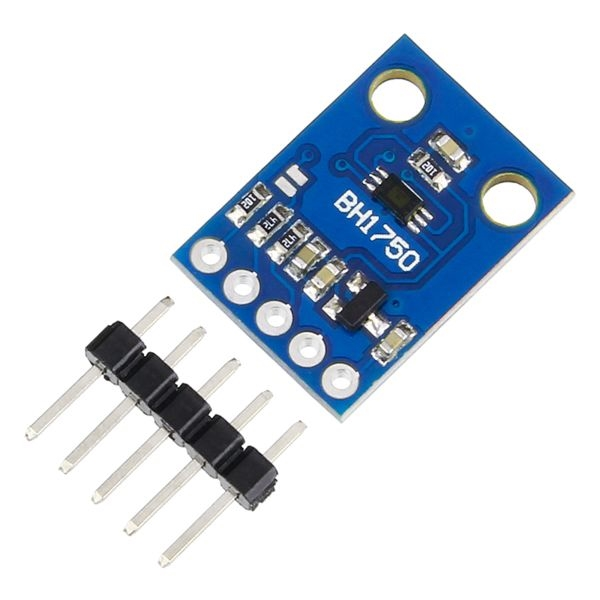
\includegraphics[scale=0.2]{figs/BH1750FVI.jpeg}
			\caption{
				سنسور روشنایی \lr{BH1750FVI}
			}
			\label{fig:schema}
		\end{figure}
		
		\begin{figure}[H]
			\centering
			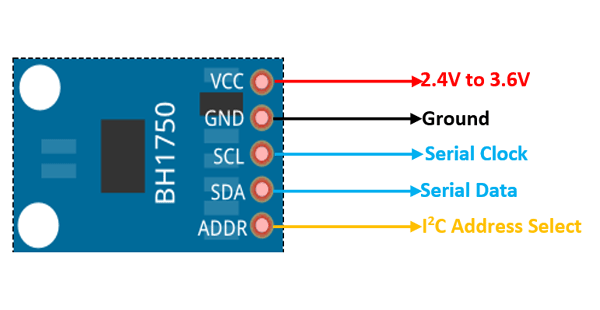
\includegraphics[scale=0.3]{figs/BH1750-Light-Sensor-Pinout.png}
			\caption{
				شرح پین‌های \lr{BH1750FVI}
			}
			\label{fig:schema}
		\end{figure}
		
		\begin{figure}[H]
			\centering
			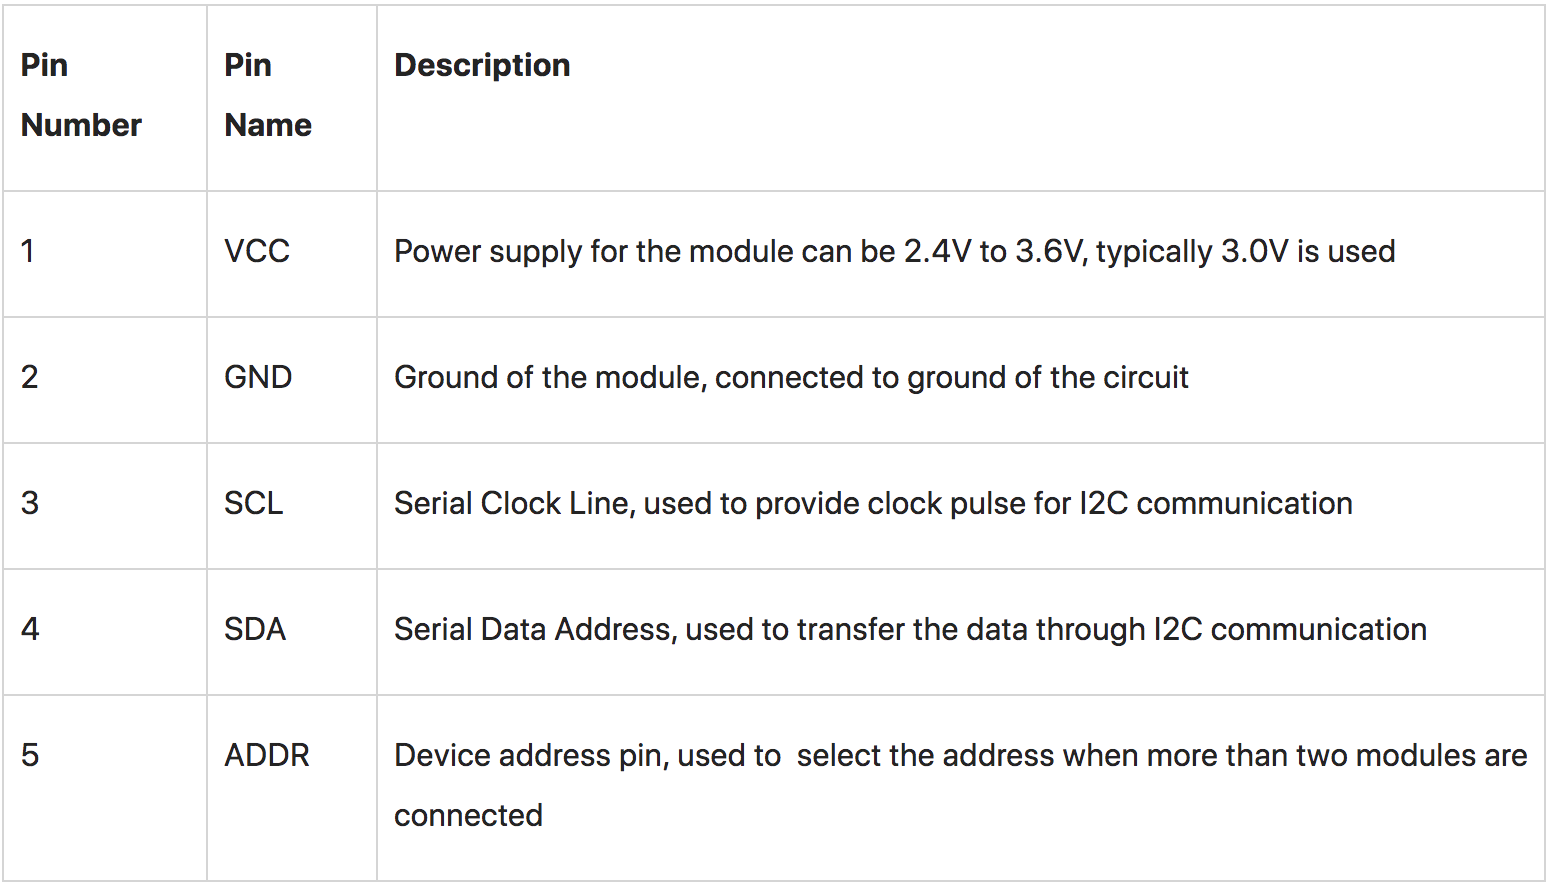
\includegraphics[scale=0.4]{figs/BH1750FVI-pin-config.png}
			\caption{
				تنظیمات پین‌های \lr{BH1750FVI}
			}
			\label{fig:schema}
		\end{figure}	
		
		\item {
			برد آردویینو مگا : \lr{Arduino Mega 2560 R3}
		}
		
		\begin{figure}[H]
			\centering
			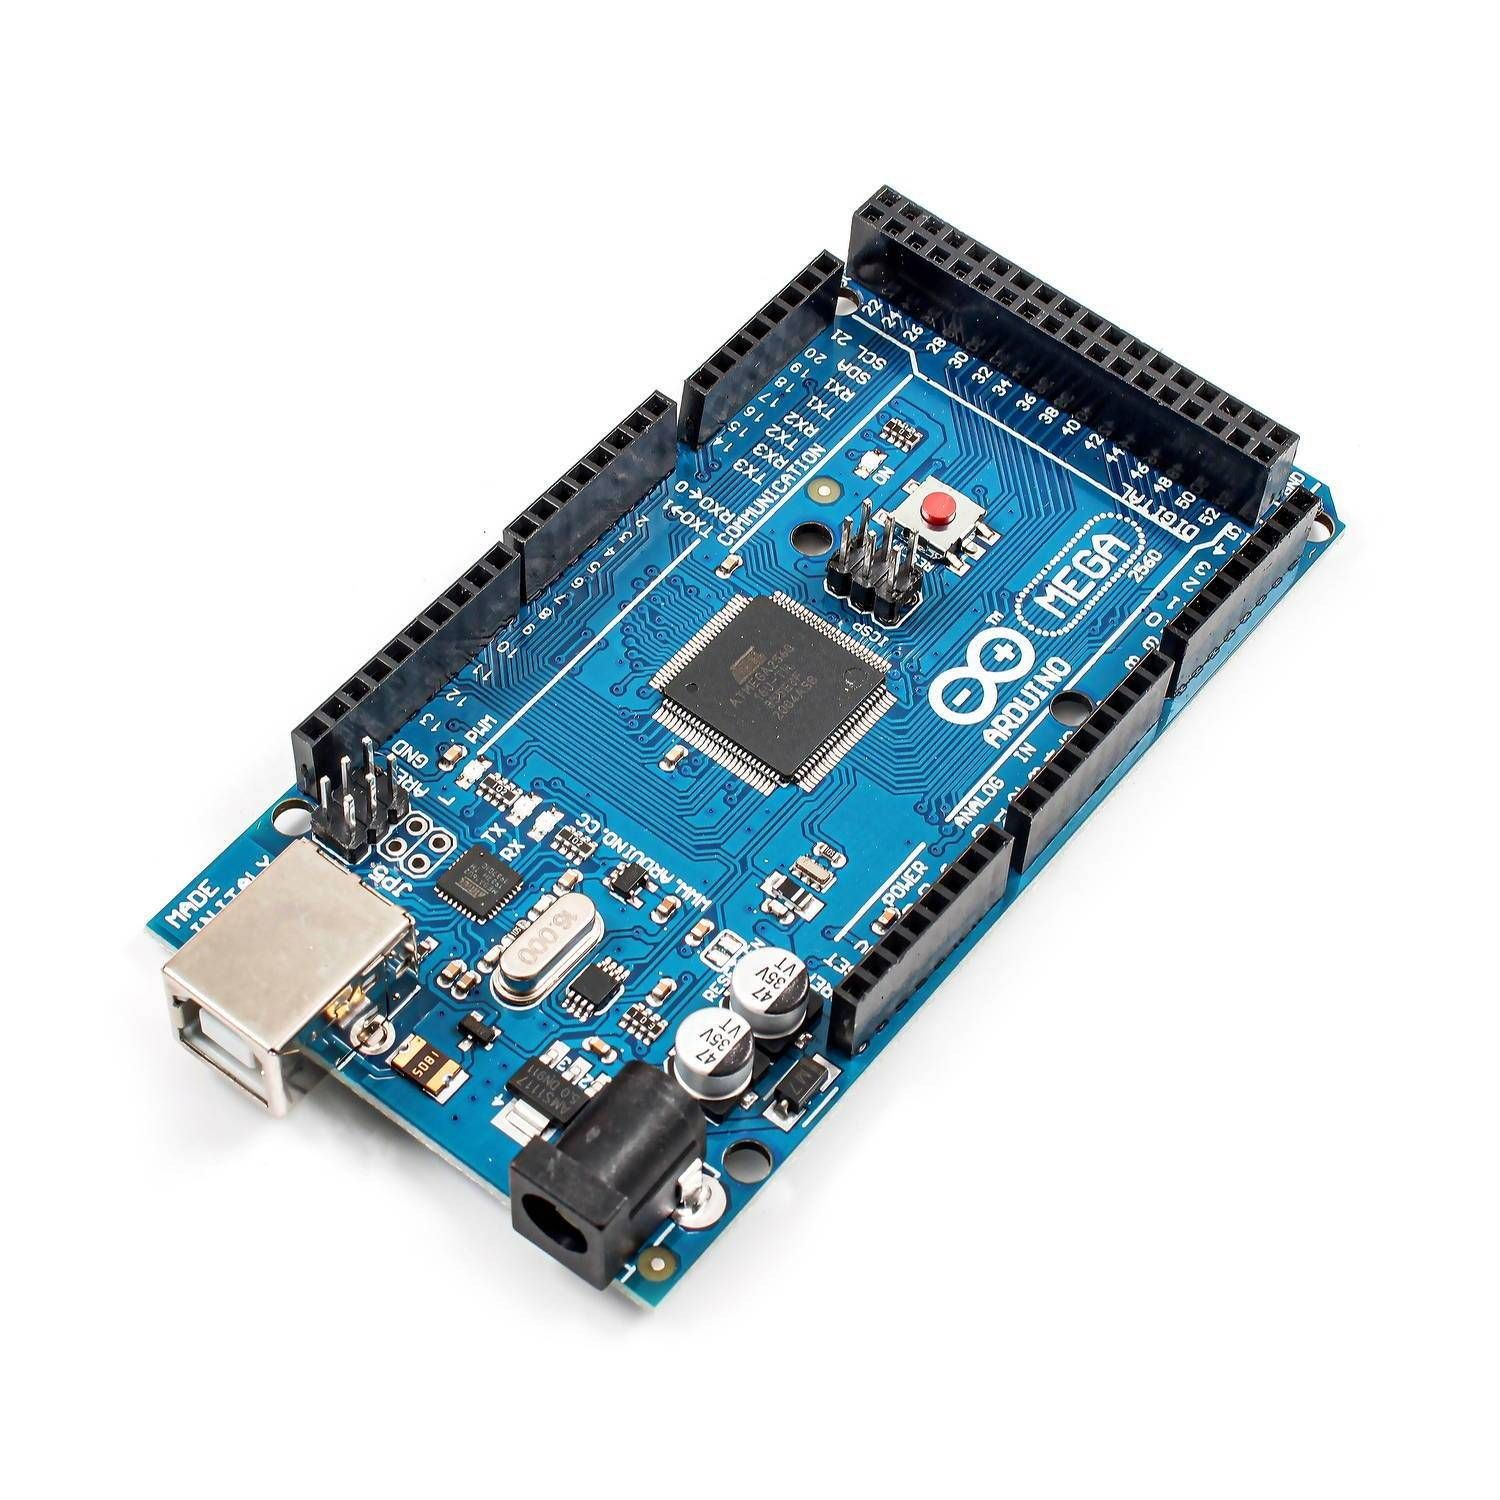
\includegraphics[scale=0.1]{figs/ard-mega.jpeg}
			\caption{
				برد \lr{Arduino Mega 2560 R3}
			}
			\label{fig:schema}
		\end{figure}
		
		\begin{figure}[H]
			\centering
			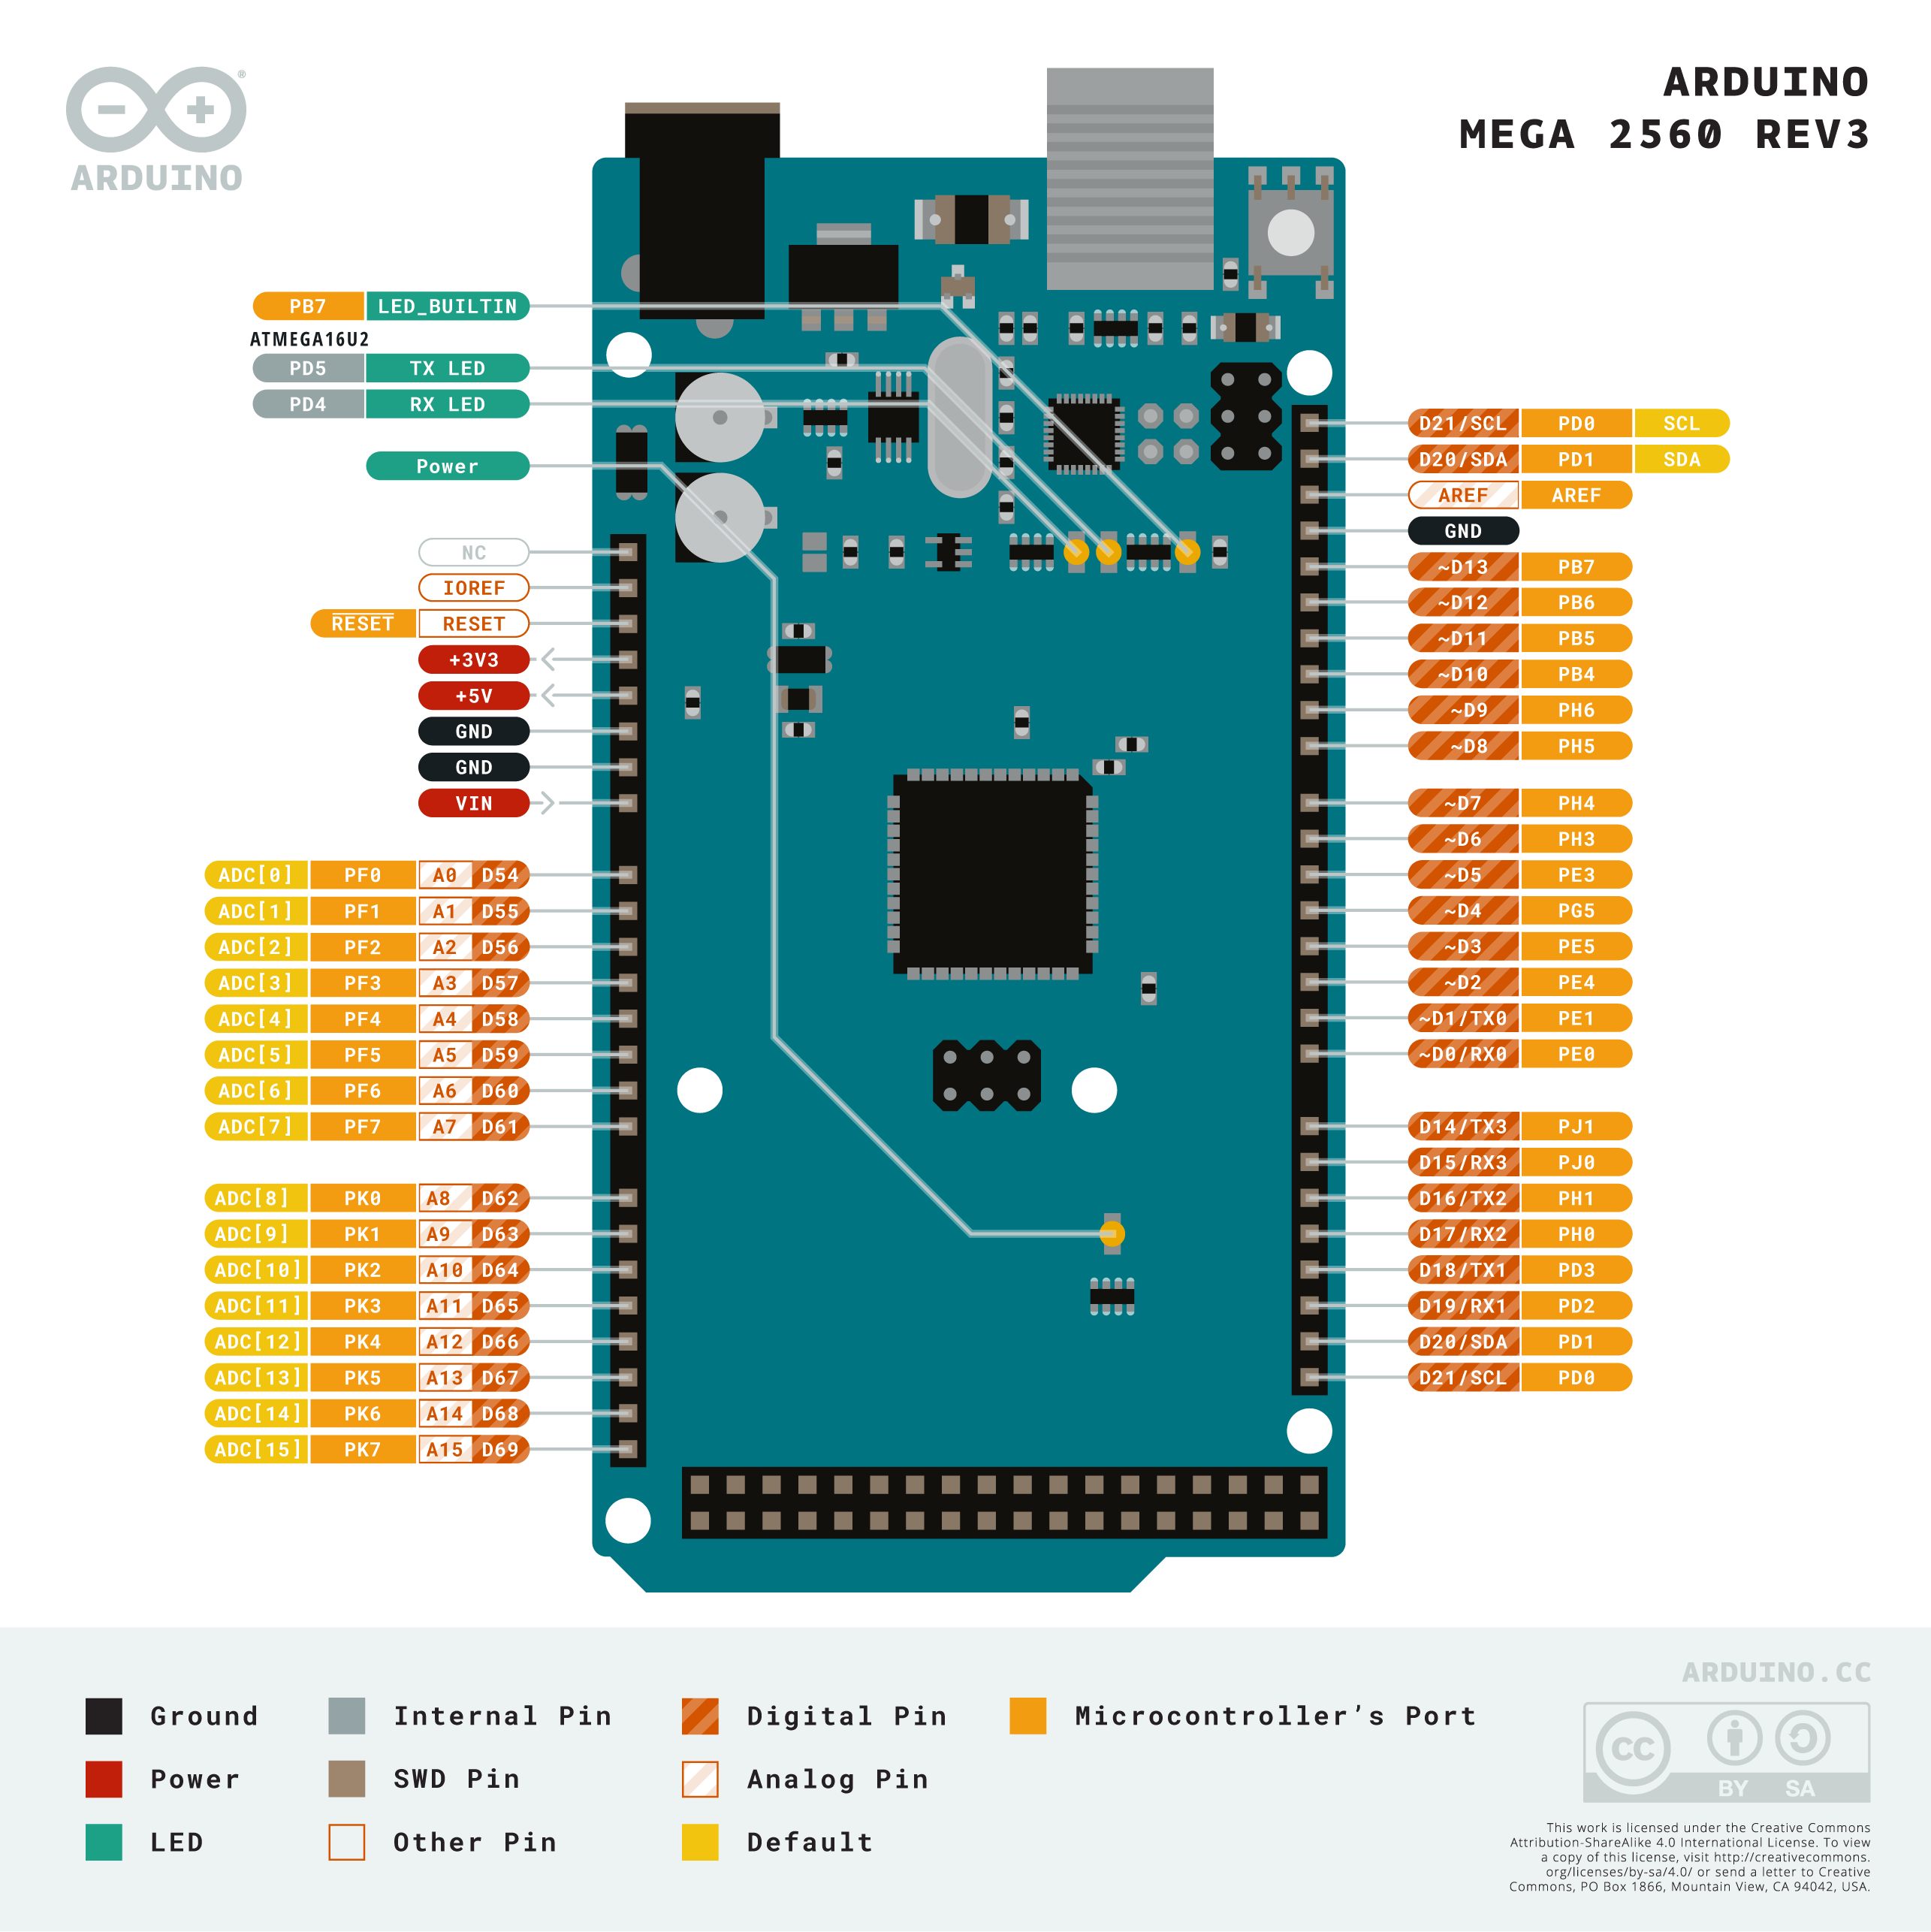
\includegraphics[scale=0.4]{figs/Pinout-Mega2560rev3-latest.png}
			\caption{
				شرح پین‌های \lr{Arduino Mega 2560 R3}
			}
			\label{fig:schema}
		\end{figure}
		
		\item {
			ماژول وای‌فای : \lr{ESP8266 ESP-01S}
			\footnote{
					این ماژول می‌تواند هم به عنوان یک نقطه دسترسی و هم به عنوان یک ایستگاه متصل به وای‌فای کار کند، بنابراین به راحتی داده‌ها را واکشی کرده و در اینترنت آپلود کند. همچنین می‌تواند با استفاده از \lr{API}، داده‌ها را از اینترنت واکشی کند و به هر اطلاعاتی که در اینترنت موجود است دسترسی داشته باشد. این ماژول فقط با ولتاژ 3.3 ولت کار می‌کند و هر ولتاژی بیش از 3.7 ولت باعث از بین رفتن ماژول می‌شود.
			}
		}
		
		\begin{figure}[H]
			\centering
			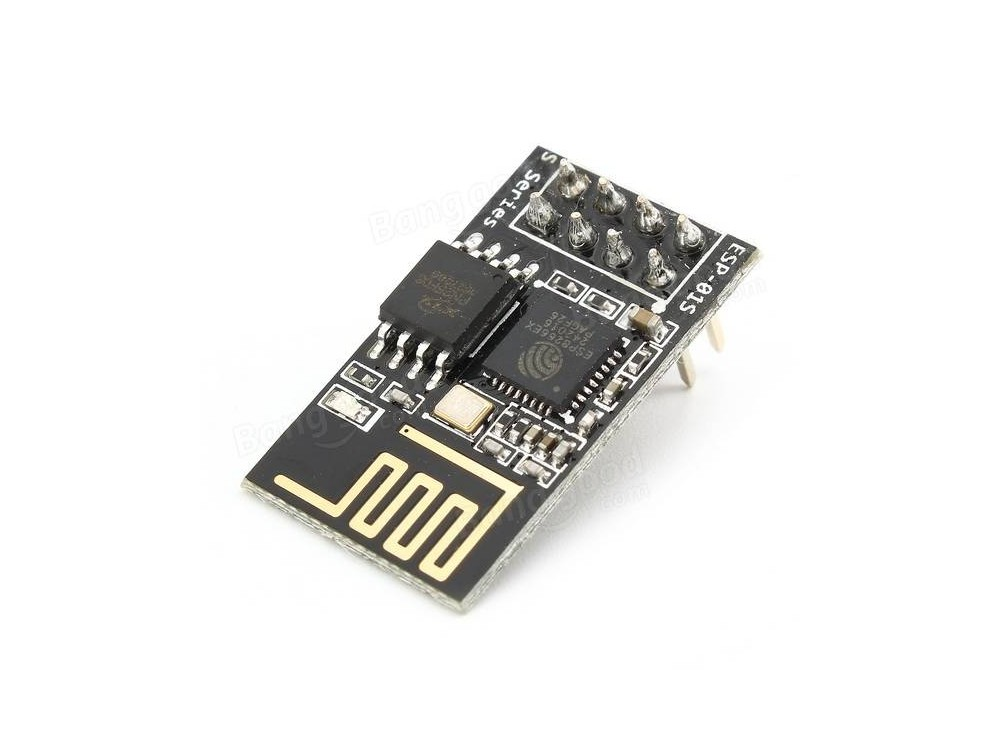
\includegraphics[scale=0.2]{figs/esp8266-esp-01s.jpeg}
			\caption{
				ماژول وای‌فای \lr{ESP8266 ESP-01S}
			}
			\label{fig:schema}
		\end{figure}
		
		\begin{figure}[H]
			\centering
			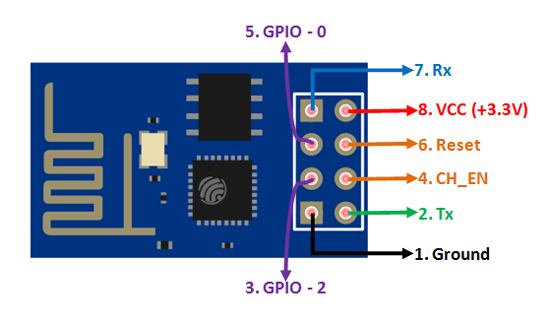
\includegraphics[scale=0.3]{figs/ESP8266-Pinout.png}
			\caption{
				شرح پین‌های \lr{ESP8266 ESP-01S}
			}
			\label{fig:schema}
		\end{figure}
		
		\begin{figure}[H]
			\centering
			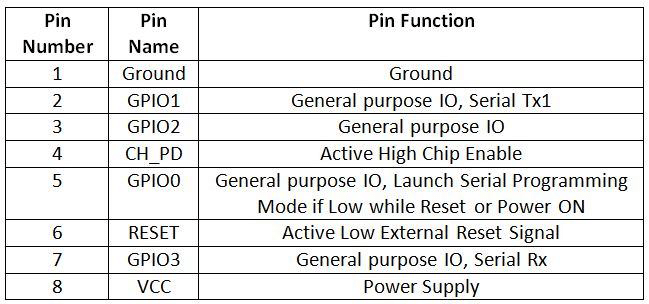
\includegraphics[scale=0.4]{figs/ESP-01-pin-configuration-The-RESET-and-VCC-pins-of-the-module-are-connected-to-the-33-V.png}
			\caption{
				تنظیمات پین‌های \lr{ESP8266 ESP-01S} (در اینجا پین \lr{GPIO1} همان \lr{TX} و \lr{GPIO3} همان \lr{TX} است. همچنین \lr{CH\_PD} معادل \lr{CH\_EN} در شرح پین است. )
			}
			\label{fig:schema}
		\end{figure}	
		
		\item {
			ترانزیستور : \lr{MOSFET IRF640}
			\footnote{
				
					ماژول \lr{IRF640} یک ماسفت با $N$ کانال است که برای اهداف سوئیچینگ با سرعت بالا طراحی شده است. این قابلیت سوئیچینگ با سرعت بالا می تواند در برنامه هایی که سرعت سوئیچینگ در آنها بسیار مهم است بسیار مفید باشد. در لوستر هوشمند، روشنایی \lr{LED} ها به سرعت توسط \lr{PWM} تغییر کند. در اینجا با توجه به اینکه منبع ولتاژ خارجی است (باتری)، باید از یک ماسفت استفاده کنیم.
				}}
		
		\begin{figure}[H]
			\centering
			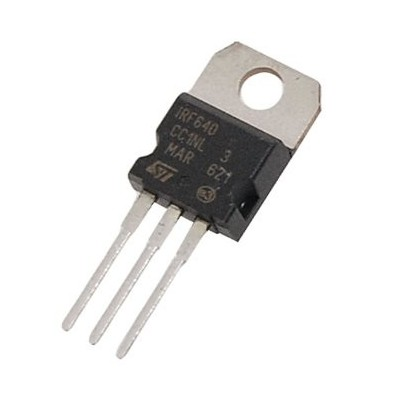
\includegraphics[scale=0.2]{figs/irf640.jpeg}
			\caption{
				ترانزیستور \lr{MOSFET IRF640}
			}
			\label{fig:schema}
		\end{figure}
		
		\begin{figure}[H]
			\centering
			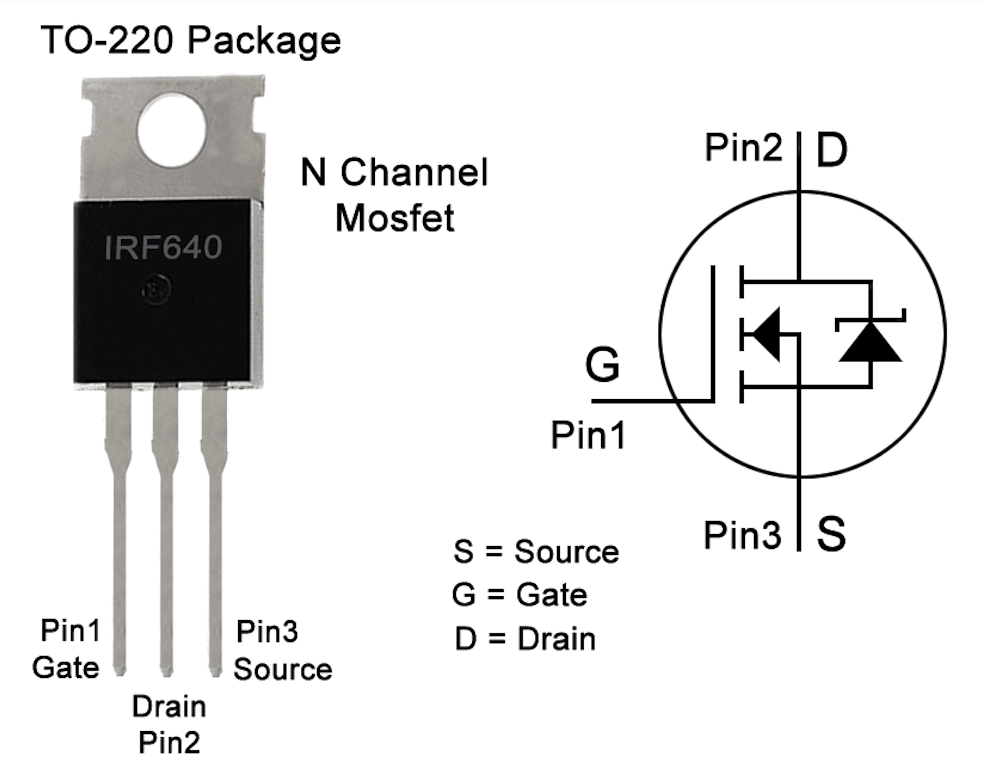
\includegraphics[scale=0.3]{figs/irf-pinout.png}
			\caption{
				ترانزیستور \lr{MOSFET IRF640}
			}
			\label{fig:schema}
		\end{figure}
			
	\end{enumerate}
	
	\newpage
	\section{طراحی مدار}
	مدار نهایی لوستر هوشمند در طی سه مرحله طراحی شده‌است. در مرحله اول مدار سنسور روشنایی بسته شد تا بتوانیم روشنایی تعداد کمی \lr{LED} را تحت تاثیر نور محیط تغییر دهیم. در مرحله دوم دو شاخه ۲۰ تایی از \lr{LED} ها را متصل کرده و به کمک منبع خارجی روشن می‌کنیم. در آخرین مرحله ماژول وای‌فای را برای برقراری ارتباط میان برنامه موبایل و آردویینو وصل می‌کنیم. هر کدام از مراحل به تفصیل در ادامه این بخش تشریح می‌شوند.
	
	\begin{enumerate}
\item اتصال سنسور روشنایی:
در این مرحله ماژول 
\lr{BH1750}
برای تشخیص نور را بورد آردویینو طبق شکل زیر وصل می‌کنیم. همانطور که مشاهده می‌شود، پورت‌های
\lr{SCL}
و
\lr{SDA}
به پورت مربوطه با همان اسم در آردویینو متصل شده‌اند. 
\lr{VCC}
را به ۵ ولت و 
\lr{ADO}
و
\lr{GND}
را به زمین متصل کردیم.
 \begin{figure}[H]
	\centering
	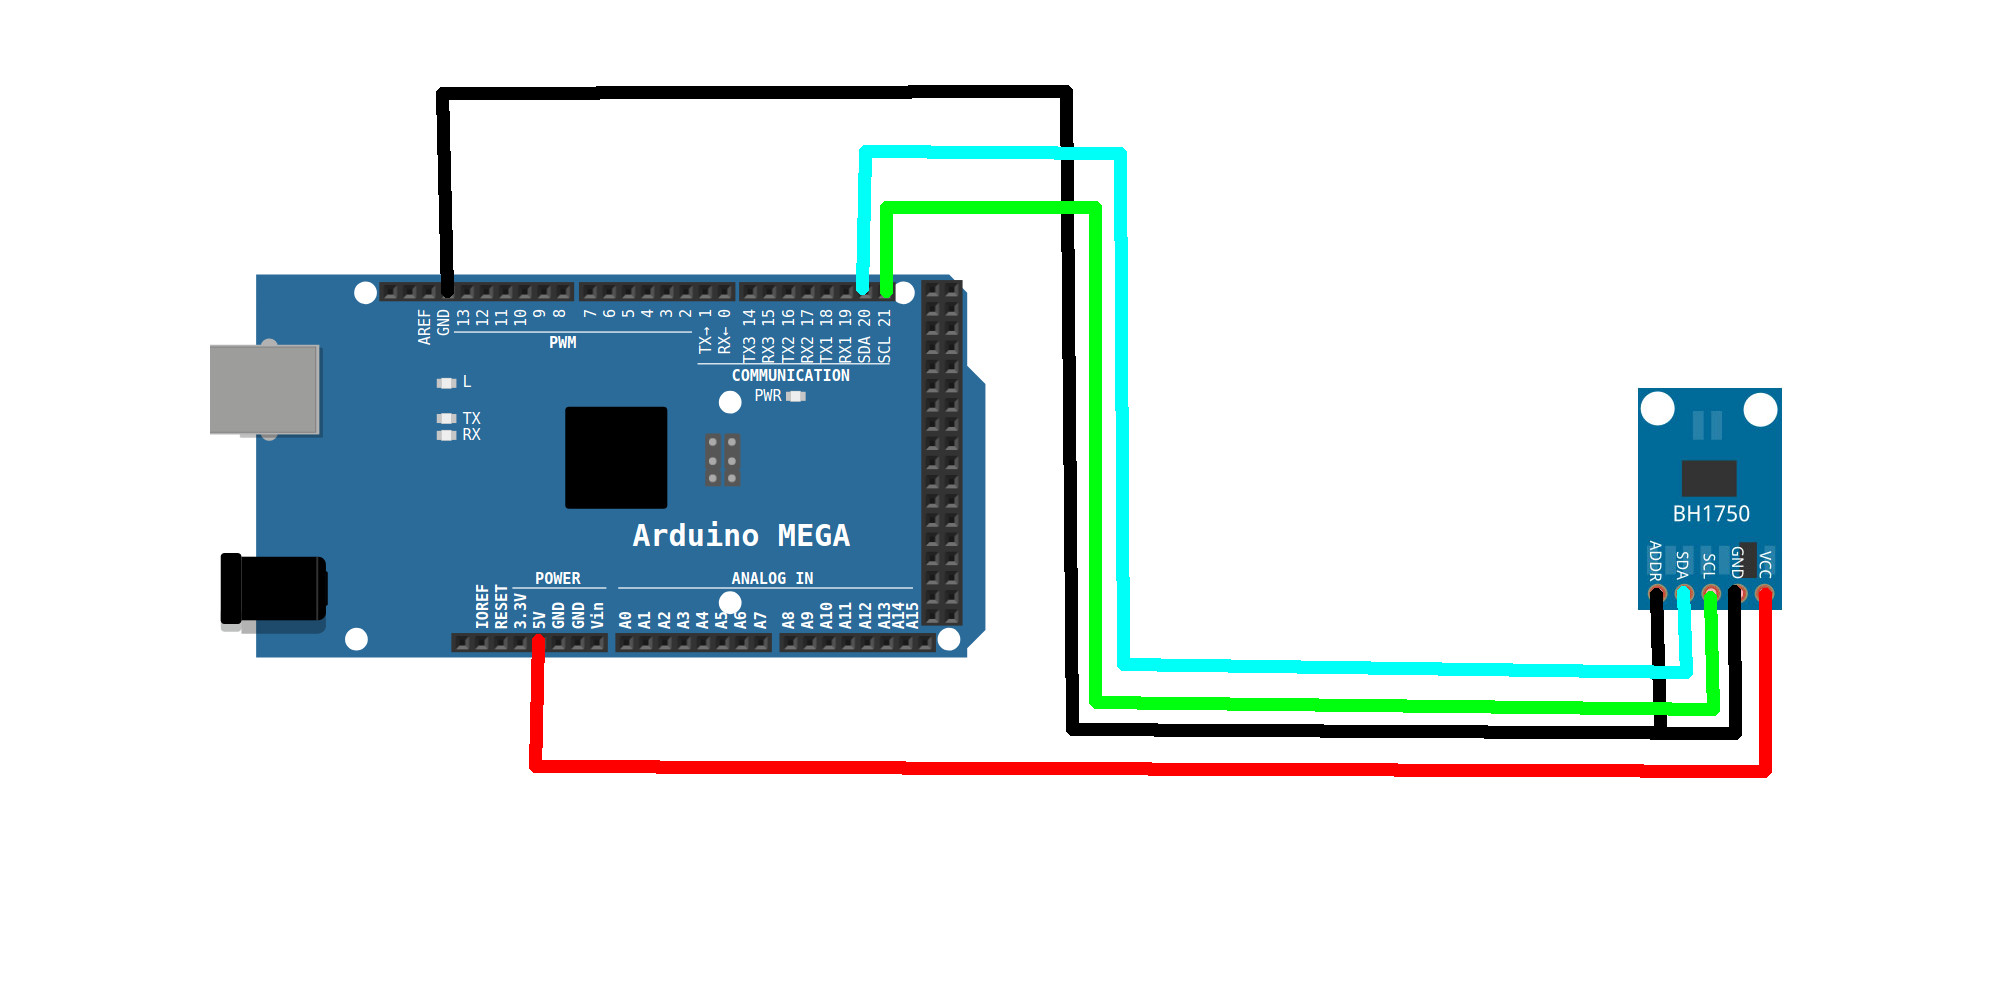
\includegraphics[scale=0.25]{figs/schema.jpg}
	\caption{
		شماتیک مدار تشخیص نور.
	}
	\label{madar}
\end{figure}

با استفاده از رابطه‌ای ساده ورودی به‌دست آمده از سنسور را با فرمولی تبدیل به 
\lr{Brightness}
ای می‌کنیم که از طریق 
\lr{PWM}
قابل کنترل است. مقدار ورودی سنسور را می‌توان با عددی ممیز شناور در بازه $0$ تا 
$2^{16}$
مدل کرد. اما به علت کاربرد ما که نور محیطی است، این مقدار خروجی با استفاده از آزمایش مقداری بین $0$ و 
$500$
به دست آمد. پس از 
\lr{scale}
کردن این مقدار بین صفر و یک مقدار روشنایی خروجی را به صورت عددی اعشاری به دست آوردیم که پس از ضرب شدن در 
$255$
به ما عدد روشنایی 
\lr{LED}
ها را می‌دهد. 

\item 
اتصال ۴۰ \lr{LED} برای شبیه‌سازی عملکرد لوستر:
هدف از این آزمایش این مرحله، بستن یک لوستر شامل ۴۰ قطعه \lr{LED}، اتصال آن به منبع خارجی، همچنین کنترل آن با ترانزیستور و در نهایت تقسیم ۴۰ \lr{LED} به دو شاخه مستقل از هم است.

ابتدا، مدار آردویینو شامل سنسور مرحله قبل را بر اساس شماتیک زیر تکمیل می‌کنیم. از ترانزیستور \lr{MOSFET IRF640} برای کنترل و یک باتری ۵ ولتی به عنوان منبع خارجی استفاده می‌کنیم.

\begin{figure}[H]
	\centering
	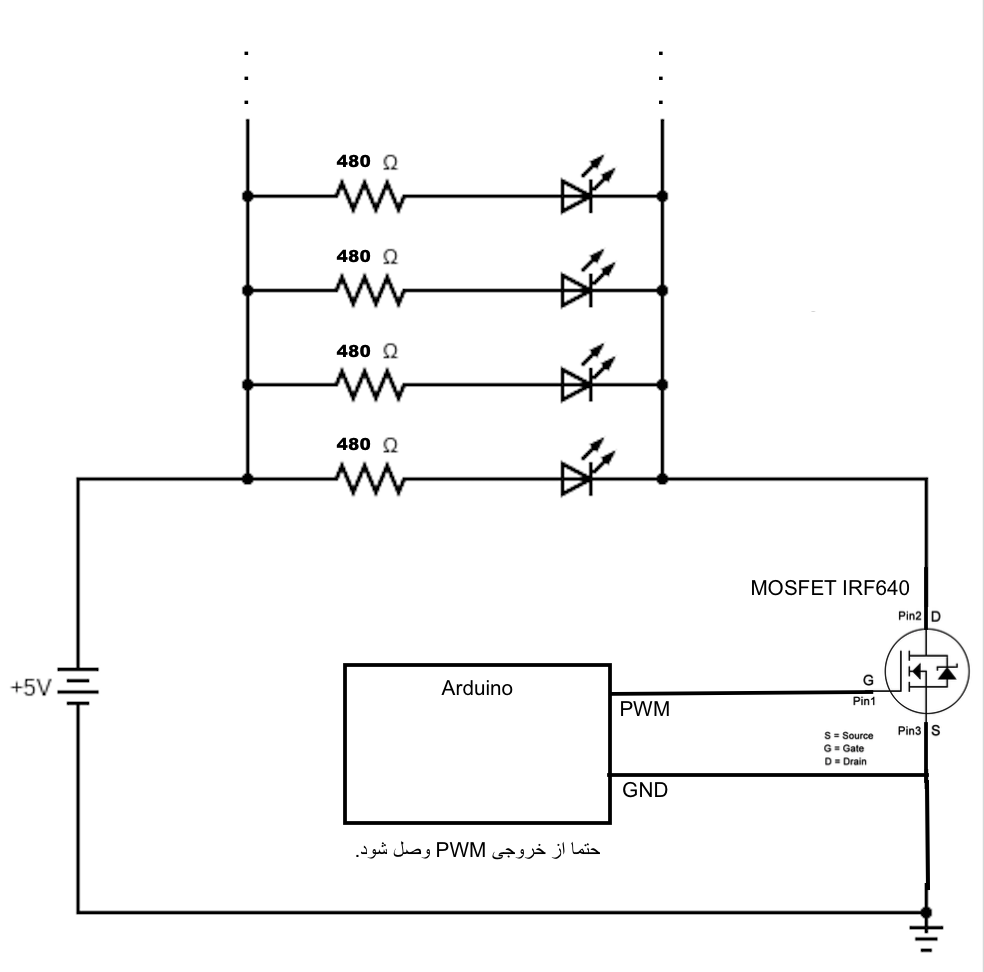
\includegraphics[scale=0.7]{figs/schematics.png}
	\caption{
		شماتیک مدار اتصال ۲۰ \lr{LED} موجود در یک شاخه. هرکدام از شاخه به یکی از پین‌های \lr{PWM} شماره ۶ یا ۷ آردویینو متصل می‌شوند.
	}
	\label{fig:schema}
\end{figure}



در این مدار، \lr{LED} ها به باتری وصل هستند و خروجی \lr{PWM} به گیت کنترل ترانزیستور \lr{MOSFET IRF640} متصل است. می‌دانیم که \lr{PWM} به کمک روشن و خاموش کردن سریع می‌تواند روشنایی را کنترل کند. در اینجا، بجای اتصال مستقیم \lr{PWM} به \lr{LED} ها، به گیت ترانزیستور متصل شده و آن را به سرعت قطع و وصل می‌کند. یعنی ترانزیستوری میان باتری و \lr{LED} است که سرعت قطع و وصل کردن آن با \lr{PWM} تنظیم می‌شود.
\item اتصال ماژول وای‌فای: 
	برای ارتباط میان موبایل اپ و آردوییو به کمک ماژول وای‌فای \lr{ESP8266 ESP-01S}، مدار را در مراحل زیر تکمیل می‌کنیم (دقت کنید که هنگام آپلود کردن کد باید پین‌های \lr{RX} و \lr{TX} قطع شوند):
	\begin{enumerate}
		\item
		پین \lr{RX} در ماژول \lr{ESP} را به پین \lr{TX} آردویینو متصل می‌کنیم.
		\item
		پین \lr{TX} در ماژول \lr{ESP} را به پین \lr{RX} آردویینو متصل می‌کنیم.
		\item
		پین \lr{CH\_PD} یا \lr{Enable} در ماژول \lr{ESP} را به پین \lr{+3V} آردویینو متصل می‌کنیم.
		\item
		پین \lr{VCC} در ماژول \lr{ESP} را به پین \lr{+3V} آردویینو متصل می‌کنیم.
	\end{enumerate}
		\end{enumerate}
	
	\newpage
\section{برنامه موبایل}
متناسب به قابلیت‌های لوستر، یک برنامه موبایل طراحی کرده‌ایم که بتوان در آن تنظیمات نام‌برده مربوط به لوستر هوشمند را انجام داد. شماتیک برنامه به شکل زیر است:

	\begin{figure}[H]
	\centering
	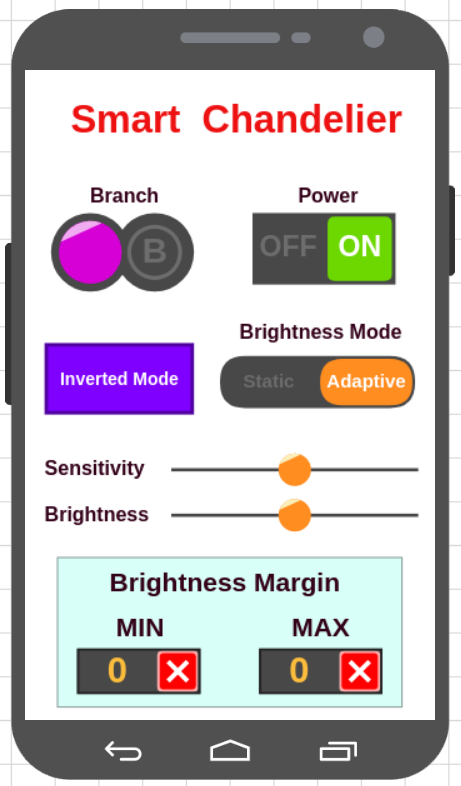
\includegraphics[scale=0.5]{figs/shcema-ma.png}
	\caption{
		شماتیک اپلیکیشن موبایل
	}
	\label{fig:schema}
\end{figure}
در نهایت می‌توان با نصب کردن برنامه موبایل و اتصال آن به \lr{ESP} و آردویینو، تنظیمات موردنظر را انجام داد. این تنظیمات و گزینه‌های موجود در این موبایل اپ به شرح زیر است:
	\begin{itemize}
		\item 
		{تنظیم حساسیت سنسور نوری:} کاربر می‌تواند با انتخاب عددی میان ۱۰ الی ۱۵۰ (توسط \lr{slidebar})، میزان حساسیت سنسور نور را تنظیم کند (عدد کمتر معادل حساسیت کمتر است؛ یعنی میزان نور با تغییرات بیشتری نسبت به عددی بیشتر تغییر می‌کند).
		\item 
		{دکمه روشن و خاموش:} کاربر می‌تواند تمامی چراغ‌های لوستر (شاخه مورد نظر) را خاموش یا روشن کند.
		\item 
		{انتخاب شاخه:} کاربر می‌تواند انتخاب کند که متغیرهای تغییر داده شده، مربوط به کدام شاخه باشند (هر شاخه، مستقل از شاخه دیگر حالت‌های مختلف و دکمه‌های متفاوت دارد).
		\item 
		{حالت استاتیک یا داینامیک (\lr{Adaptive}):} کاربر می‌تواند با حالت استاتیک یک مقدار خاص را برای روشنایی انتخاب کرده و تمامی \lr{LED} های لوستر با آن مقدار تنظیم می‌شوند. در حالت داینامیک نیز مقدار روشنایی لوستر با سنسورهای تنظیم می‌شود.
		\item 
		{تنظیم حداکثر و حداقل میزان روشنایی:} کاربر می‌تواند با انتخاب عددی میان ۰ تا ۲۵۵(توسط \lr{slidebar})، حداقل و حداکثر میزان روشنایی یک شاخه را تعیین کند. بنابراین روشنایی یک شاخه، محدود به این دو عدد می‌شود و نمی‌تواند مقداری خارج از این بازه بگیرد.
		\item 
		{مودهای مختلف لوستر:} مودهای متفاوت که می‌توانند شامل لوستر را در حالت تنظیم داینامیک عادی یا رقص نور (همانند گزارش اول) تنظیم کنند (این حالت‌ها در قسمت‌های بعدی تکمیل می‌شوند). یکی از مودهای در نظر گرفته شده برای این قسمت حالت \lr{Inverted min to max} است که در آن نور دو شاخه به صورت معکوس با همدیگر کم و زیاد می‌شود.
		
	\end{itemize}
\newpage
	\section{توضیحات کد}
	
	بخش اولیه کد شامل ورودی‌هایی است که کاربر از طریق 
\lr{UI}
وارد می‌کند و همانطور که در شکل زیر می‌بینید در قالب فرمت
\lr{struct}
آمده‌است:

\begin{latin}
	\lstinputlisting[style={verilog-style}]{src/remotexyStruct.ino}
\end{latin}

این ورودی‌ در بخش حلقه اصلی کد به ازای شاخه انتخابی در یک ساختار
\lr{Config}
به ازای هر شاخه ذخیره می‌شوند. ساختار 
\lr{Config}
به ازای هر شاخه یک زیر نوع به فرم زیر است.
\begin{latin}
	\lstinputlisting[style={verilog-style}]{src/branchConfigs.ino}
\end{latin}

در ابتدای کار این مقادیر به صورت زیر مقداردهی اولیه می‌شوند.
\begin{latin}
	\lstinputlisting[style={verilog-style}]{src/setupConf.ino}
\end{latin}
و به صورت زیر در هر مرحله مقادیر ورودی شاخه از طریق 
\lr{UI}
به ازای شاخه مورد نظر وارد می‌شود. لازم به ذکر است که برنامه به نحوی زده شده که اگر بیشتر از دو شاخه نیز داشته باشیم باز هم بدون هیچ مشکلی کار کند. 

\begin{latin}
	\lstinputlisting[style={verilog-style}]{src/mainLoopSetupConf.ino}
\end{latin}

توجه کنید اگر مقدار
\lr{conf-activated}
به ازای یکی از شاخه‌ها غیر فعال باشد یعنی در حلقه اصلی مقدار خروجی این شاخه از روی شاخه‌های دیگر محاسبه می‌شود و لازم به مقدار دهی آن نیستیم. توجه کنید اگر شاخه‌ای شاخه قبلش روی حالت 
\lr{inverted}
تنظیم شده باشد یعنی این شاخه و قبلی به صورت رقص نور و سنکرون باهم تغییر می‌کنند و شاخه قبلی مقدار خروحی این شاخه را تنظیم می‌کند.


در بخش بعدی از حلقه اصلی روی تمامی شاخه‌ها پیمایش می‌کنیم و به ازای شاخه‌هایی که باید مقدار خروجی‌شان را تعیین کنیم بر اساس مقادیر داده شده در
\lr{branch-conf}
مقدار خروجی این پین را تنظیم می‌کنیم.

مقدار خروجی بر اساس ورودی بر اساس چهار تا از پارامتر‌های کانفیگ هر شاخه تنظیم می‌شود:
\begin{itemize}
	\item 
	اگر مقدار
	\lr{conf.power}
	برابر با صفر باشد یعنی این شاخه غیر فعال شده و در نتیجه مقدار خروجی‌ آن مستقل از هر چیز دیگری برابر صفر است.
	
	\item 
	مقدار
	\lr{conf.brightness-mode}
	به شاخه می‌گوید که ورودی سنسور را در این شاخه لحاظ کنیم یا نه. در صورتیکه این مقدار صفر باشد، مقدار خروجی برابر
	\lr{conf.min}
	خواهد بود و در صورتیکه برابر یک باشد به صورت 
	\lr{adaptive}
	از روی ورودی سنسور خروجی‌اش تنظیم می‌شود. مقدار خروجی بر اساس ورودی سنسور یک تابع خطی است. ابتدا تابع زیر را در نظر بگیرید که اسکیل کردن یک مقدار
	\lr{ratio}
	بین دو بازه استفاده می‌شود.
	$$scale(l, x, r) = (1 - x) \times l + x \times r$$
	 و مطابق با فرمول زیر مقدار ورودی سنسور را تبدیل به عددی بین صفر و یک می‌کنیم
	$$b = 1 - \min(1, \frac{x}{scale(s_{\min} , s , s_{\max})})$$
	این خروجی باید بین 
	\lr{brightness-max}
	و
	\lr{brightness-min}
	تنظیم شود و به صورت زیر این‌کار انجام می‌شود.
	$$out = scale(brightness_{\min}, b, brightness_{\max})$$
	
	توجه کنید به ازای این کد خاص مقدار
	$s_{\min}$
	و
	$s_{\max}$
	به ترتیب برابر ۱۰ و ۱۵۰ شده‌اند که محدوده بیشترین نور و کمترین نور در اتاق محل آزمایش است. همچنین مقدار
	$s$
	نیز یک پارامتر قابل تنظیم است که از طریق ورودی 
	\lr{UI}
	و مقدار
	\lr{conf.sensitivity}
	تنظیم می‌شود.
	\item
	مقدار 
	\lr{conf.inverted-mode}
	برابر صفر یا یک است که اگر برابر یک باشد یعنی این شاخه و شاخه بعدی رقص نور انجام می‌دهند. برای پیاده‌سازی این رقص نور مقدار خروجی آیتم بعدی که برابر با
	$out$
	بود را در نظر می‌گیریم و به ترتیب مقدار این شاخه و بعدی اش را مطابق دنباله زیر تنظیم می‌کنیم:
	$$<(\frac{out}{2}, \frac{out}{2}), (\frac{out}{2} + 1, \frac{out}{2} - 1), (\frac{out}{2} + 2, \frac{out}{2} - 2) ... >$$
	برای اینکه فرمت خروجی پویا باشد از یک پارامتر شمارنده به اسم
	\lr{nxt-branch-counter}
	بهره بردیم و این مقدار هر سری در بین بازه‌ای معقول قرار می‌گیرد و به شاخه اول اضافه می‌شود و از شاخه دوم کم می‌شود. به این ترتیب همیشه جمع اندازه خروجی این دو شاخه متوالی برابر با مقدار خروجی‌ای‌است که به ازای شاخه اولی تنظیم شده‌بود.
\end{itemize}

برای اطلاعات بیشتر از بخش‌های کد می‌توانید سورس کامل را در پیوست های پروژه به همراه مستندات کامل مشاهده نمایید.


	
	%\begin{latin}
	%	\lstinputlisting[style={verilog-style}]{src/project.ino}
	%\end{latin}
	
	\newpage
	\section*{جمع‌بندی}
در این پروژه قصد داشتیم که یک  لوستر هوشمند طراحی کنیم که بتواند با توجه به نیازمندی‌های کاربر روشنایی دو اتاق در خانه را شبیه‌سازی کند. کاربر می‌تواند بوسیله برنامه موبایل و به طریق بی‌سیم از میان حالت‌های ارائه شده انتخاب کند یا تنظیمات خودش را اعمال نماید. برای ادامه دادن این کار می‌توان تنظیمات ساعت‌های روشنایی را طبق برنامه کاربر نیز به برنامه اضافه کرد.
	
\end{document}